\documentclass[AMA,LATO1COL]{WileyNJD-v2}
% Text begins on line 369
    
    \usepackage[breakable]{tcolorbox}
    \tcbset{nobeforeafter} % prevents tcolorboxes being placing in paragraphs
    \usepackage{float}
    \floatplacement{figure}{H} % forces figures to be placed at the correct location
    
    \usepackage[T1]{fontenc}
    % Nicer default font (+ math font) than Computer Modern for most use cases
    \usepackage{mathpazo}

    % Basic figure setup, for now with no caption control since it's done
    % automatically by Pandoc (which extracts ![](path) syntax from Markdown).
    \usepackage{graphicx}
    % We will generate all images so they have a width \maxwidth. This means
    % that they will get their normal width if they fit onto the page, but
    % are scaled down if they would overflow the margins.
    \makeatletter
    \def\maxwidth{\ifdim\Gin@nat@width>\linewidth\linewidth
    \else\Gin@nat@width\fi}
    \makeatother
    \let\Oldincludegraphics\includegraphics
    % Set max figure width to be 80% of text width, for now hardcoded.
    % \renewcommand{\includegraphics}[1]{\Oldincludegraphics[width=.8\maxwidth]{#1}}
    % Ensure that by default, figures have no caption (until we provide a
    % proper Figure object with a Caption API and a way to capture that
    % in the conversion process - todo).
    \usepackage{caption}
    \DeclareCaptionLabelFormat{nolabel}{}
    \captionsetup{labelformat=nolabel}

    \usepackage{adjustbox} % Used to constrain images to a maximum size 
    \usepackage{xcolor} % Allow colors to be defined
    \usepackage{enumerate} % Needed for markdown enumerations to work
    \usepackage{geometry} % Used to adjust the document margins
    \usepackage{amsmath} % Equations
    \usepackage{amssymb} % Equations
    \usepackage{textcomp} % defines textquotesingle
    % Hack from http://tex.stackexchange.com/a/47451/13684:
    \AtBeginDocument{%
        \def\PYZsq{\textquotesingle}% Upright quotes in Pygmentized code
    }
    \usepackage{upquote} % Upright quotes for verbatim code
    \usepackage{eurosym} % defines \euro
    \usepackage[mathletters]{ucs} % Extended unicode (utf-8) support
    \usepackage[utf8x]{inputenc} % Allow utf-8 characters in the tex document
    \usepackage{fancyvrb} % verbatim replacement that allows latex
    \usepackage{grffile} % extends the file name processing of package graphics 
                         % to support a larger range 
    % The hyperref package gives us a pdf with properly built
    % internal navigation ('pdf bookmarks' for the table of contents,
    % internal cross-reference links, web links for URLs, etc.)
    \usepackage{hyperref}
    \usepackage{longtable} % longtable support required by pandoc >1.10
    \usepackage{booktabs}  % table support for pandoc > 1.12.2
    \usepackage[inline]{enumitem} % IRkernel/repr support (it uses the enumerate* environment)
    \usepackage[normalem]{ulem} % ulem is needed to support strikethroughs (\sout)
                                % normalem makes italics be italics, not underlines
    \usepackage{mathrsfs}
    


    % defining Matlab colors
    \definecolor{pltblue}{rgb}{0.12156862745098039, 0.4666666666666667, 0.7058823529411765}
    \definecolor{pltred}{rgb}{0.8392156862745098, 0.15294117647058825, 0.1568627450980392}



    
    % Colors for the hyperref package
    \definecolor{urlcolor}{rgb}{0,.145,.698}
    \definecolor{linkcolor}{rgb}{.71,0.21,0.01}
    \definecolor{citecolor}{rgb}{.12,.54,.11}

    % ANSI colors
    \definecolor{ansi-black}{HTML}{3E424D}
    \definecolor{ansi-black-intense}{HTML}{282C36}
    \definecolor{ansi-red}{HTML}{E75C58}
    \definecolor{ansi-red-intense}{HTML}{B22B31}
    \definecolor{ansi-green}{HTML}{00A250}
    \definecolor{ansi-green-intense}{HTML}{007427}
    \definecolor{ansi-yellow}{HTML}{DDB62B}
    \definecolor{ansi-yellow-intense}{HTML}{B27D12}
    \definecolor{ansi-blue}{HTML}{208FFB}
    \definecolor{ansi-blue-intense}{HTML}{0065CA}
    \definecolor{ansi-magenta}{HTML}{D160C4}
    \definecolor{ansi-magenta-intense}{HTML}{A03196}
    \definecolor{ansi-cyan}{HTML}{60C6C8}
    \definecolor{ansi-cyan-intense}{HTML}{258F8F}
    \definecolor{ansi-white}{HTML}{C5C1B4}
    \definecolor{ansi-white-intense}{HTML}{A1A6B2}
    \definecolor{ansi-default-inverse-fg}{HTML}{FFFFFF}
    \definecolor{ansi-default-inverse-bg}{HTML}{000000}

    % commands and environments needed by pandoc snippets
    % extracted from the output of `pandoc -s`
    \providecommand{\tightlist}{%
      \setlength{\itemsep}{0pt}\setlength{\parskip}{0pt}}
    \DefineVerbatimEnvironment{Highlighting}{Verbatim}{commandchars=\\\{\}}
    % Add ',fontsize=\small' for more characters per line
    \newenvironment{Shaded}{}{}
    \newcommand{\KeywordTok}[1]{\textcolor[rgb]{0.00,0.44,0.13}{\textbf{{#1}}}}
    \newcommand{\DataTypeTok}[1]{\textcolor[rgb]{0.56,0.13,0.00}{{#1}}}
    \newcommand{\DecValTok}[1]{\textcolor[rgb]{0.25,0.63,0.44}{{#1}}}
    \newcommand{\BaseNTok}[1]{\textcolor[rgb]{0.25,0.63,0.44}{{#1}}}
    \newcommand{\FloatTok}[1]{\textcolor[rgb]{0.25,0.63,0.44}{{#1}}}
    \newcommand{\CharTok}[1]{\textcolor[rgb]{0.25,0.44,0.63}{{#1}}}
    \newcommand{\StringTok}[1]{\textcolor[rgb]{0.25,0.44,0.63}{{#1}}}
    \newcommand{\CommentTok}[1]{\textcolor[rgb]{0.38,0.63,0.69}{\textit{{#1}}}}
    \newcommand{\OtherTok}[1]{\textcolor[rgb]{0.00,0.44,0.13}{{#1}}}
    \newcommand{\AlertTok}[1]{\textcolor[rgb]{1.00,0.00,0.00}{\textbf{{#1}}}}
    \newcommand{\FunctionTok}[1]{\textcolor[rgb]{0.02,0.16,0.49}{{#1}}}
    \newcommand{\RegionMarkerTok}[1]{{#1}}
    \newcommand{\ErrorTok}[1]{\textcolor[rgb]{1.00,0.00,0.00}{\textbf{{#1}}}}
    \newcommand{\NormalTok}[1]{{#1}}
    
    % Additional commands for more recent versions of Pandoc
    \newcommand{\ConstantTok}[1]{\textcolor[rgb]{0.53,0.00,0.00}{{#1}}}
    \newcommand{\SpecialCharTok}[1]{\textcolor[rgb]{0.25,0.44,0.63}{{#1}}}
    \newcommand{\VerbatimStringTok}[1]{\textcolor[rgb]{0.25,0.44,0.63}{{#1}}}
    \newcommand{\SpecialStringTok}[1]{\textcolor[rgb]{0.73,0.40,0.53}{{#1}}}
    \newcommand{\ImportTok}[1]{{#1}}
    \newcommand{\DocumentationTok}[1]{\textcolor[rgb]{0.73,0.13,0.13}{\textit{{#1}}}}
    \newcommand{\AnnotationTok}[1]{\textcolor[rgb]{0.38,0.63,0.69}{\textbf{\textit{{#1}}}}}
    \newcommand{\CommentVarTok}[1]{\textcolor[rgb]{0.38,0.63,0.69}{\textbf{\textit{{#1}}}}}
    \newcommand{\VariableTok}[1]{\textcolor[rgb]{0.10,0.09,0.49}{{#1}}}
    \newcommand{\ControlFlowTok}[1]{\textcolor[rgb]{0.00,0.44,0.13}{\textbf{{#1}}}}
    \newcommand{\OperatorTok}[1]{\textcolor[rgb]{0.40,0.40,0.40}{{#1}}}
    \newcommand{\BuiltInTok}[1]{{#1}}
    \newcommand{\ExtensionTok}[1]{{#1}}
    \newcommand{\PreprocessorTok}[1]{\textcolor[rgb]{0.74,0.48,0.00}{{#1}}}
    \newcommand{\AttributeTok}[1]{\textcolor[rgb]{0.49,0.56,0.16}{{#1}}}
    \newcommand{\InformationTok}[1]{\textcolor[rgb]{0.38,0.63,0.69}{\textbf{\textit{{#1}}}}}
    \newcommand{\WarningTok}[1]{\textcolor[rgb]{0.38,0.63,0.69}{\textbf{\textit{{#1}}}}}
    
    
    % Define a nice break command that doesn't care if a line doesn't already
    % exist.
    \def\br{\hspace*{\fill} \\* }
    % Math Jax compatibility definitions
    \def\gt{>}
    \def\lt{<}
    \let\Oldtex\TeX
    \let\Oldlatex\LaTeX
    \renewcommand{\TeX}{\textrm{\Oldtex}}
    \renewcommand{\LaTeX}{\textrm{\Oldlatex}}
    % Document parameters
    % Document title
    \title{Baseline \& Residual Water Simulator}
    
    
    
    
    
% Pygments definitions
\makeatletter
\def\PY@reset{\let\PY@it=\relax \let\PY@bf=\relax%
    \let\PY@ul=\relax \let\PY@tc=\relax%
    \let\PY@bc=\relax \let\PY@ff=\relax}
\def\PY@tok#1{\csname PY@tok@#1\endcsname}
\def\PY@toks#1+{\ifx\relax#1\empty\else%
    \PY@tok{#1}\expandafter\PY@toks\fi}
\def\PY@do#1{\PY@bc{\PY@tc{\PY@ul{%
    \PY@it{\PY@bf{\PY@ff{#1}}}}}}}
\def\PY#1#2{\PY@reset\PY@toks#1+\relax+\PY@do{#2}}

\expandafter\def\csname PY@tok@w\endcsname{\def\PY@tc##1{\textcolor[rgb]{0.73,0.73,0.73}{##1}}}
\expandafter\def\csname PY@tok@c\endcsname{\let\PY@it=\textit\def\PY@tc##1{\textcolor[rgb]{0.25,0.50,0.50}{##1}}}
\expandafter\def\csname PY@tok@cp\endcsname{\def\PY@tc##1{\textcolor[rgb]{0.74,0.48,0.00}{##1}}}
\expandafter\def\csname PY@tok@k\endcsname{\let\PY@bf=\textbf\def\PY@tc##1{\textcolor[rgb]{0.00,0.50,0.00}{##1}}}
\expandafter\def\csname PY@tok@kp\endcsname{\def\PY@tc##1{\textcolor[rgb]{0.00,0.50,0.00}{##1}}}
\expandafter\def\csname PY@tok@kt\endcsname{\def\PY@tc##1{\textcolor[rgb]{0.69,0.00,0.25}{##1}}}
\expandafter\def\csname PY@tok@o\endcsname{\def\PY@tc##1{\textcolor[rgb]{0.40,0.40,0.40}{##1}}}
\expandafter\def\csname PY@tok@ow\endcsname{\let\PY@bf=\textbf\def\PY@tc##1{\textcolor[rgb]{0.67,0.13,1.00}{##1}}}
\expandafter\def\csname PY@tok@nb\endcsname{\def\PY@tc##1{\textcolor[rgb]{0.00,0.50,0.00}{##1}}}
\expandafter\def\csname PY@tok@nf\endcsname{\def\PY@tc##1{\textcolor[rgb]{0.00,0.00,1.00}{##1}}}
\expandafter\def\csname PY@tok@nc\endcsname{\let\PY@bf=\textbf\def\PY@tc##1{\textcolor[rgb]{0.00,0.00,1.00}{##1}}}
\expandafter\def\csname PY@tok@nn\endcsname{\let\PY@bf=\textbf\def\PY@tc##1{\textcolor[rgb]{0.00,0.00,1.00}{##1}}}
\expandafter\def\csname PY@tok@ne\endcsname{\let\PY@bf=\textbf\def\PY@tc##1{\textcolor[rgb]{0.82,0.25,0.23}{##1}}}
\expandafter\def\csname PY@tok@nv\endcsname{\def\PY@tc##1{\textcolor[rgb]{0.10,0.09,0.49}{##1}}}
\expandafter\def\csname PY@tok@no\endcsname{\def\PY@tc##1{\textcolor[rgb]{0.53,0.00,0.00}{##1}}}
\expandafter\def\csname PY@tok@nl\endcsname{\def\PY@tc##1{\textcolor[rgb]{0.63,0.63,0.00}{##1}}}
\expandafter\def\csname PY@tok@ni\endcsname{\let\PY@bf=\textbf\def\PY@tc##1{\textcolor[rgb]{0.60,0.60,0.60}{##1}}}
\expandafter\def\csname PY@tok@na\endcsname{\def\PY@tc##1{\textcolor[rgb]{0.49,0.56,0.16}{##1}}}
\expandafter\def\csname PY@tok@nt\endcsname{\let\PY@bf=\textbf\def\PY@tc##1{\textcolor[rgb]{0.00,0.50,0.00}{##1}}}
\expandafter\def\csname PY@tok@nd\endcsname{\def\PY@tc##1{\textcolor[rgb]{0.67,0.13,1.00}{##1}}}
\expandafter\def\csname PY@tok@s\endcsname{\def\PY@tc##1{\textcolor[rgb]{0.73,0.13,0.13}{##1}}}
\expandafter\def\csname PY@tok@sd\endcsname{\let\PY@it=\textit\def\PY@tc##1{\textcolor[rgb]{0.73,0.13,0.13}{##1}}}
\expandafter\def\csname PY@tok@si\endcsname{\let\PY@bf=\textbf\def\PY@tc##1{\textcolor[rgb]{0.73,0.40,0.53}{##1}}}
\expandafter\def\csname PY@tok@se\endcsname{\let\PY@bf=\textbf\def\PY@tc##1{\textcolor[rgb]{0.73,0.40,0.13}{##1}}}
\expandafter\def\csname PY@tok@sr\endcsname{\def\PY@tc##1{\textcolor[rgb]{0.73,0.40,0.53}{##1}}}
\expandafter\def\csname PY@tok@ss\endcsname{\def\PY@tc##1{\textcolor[rgb]{0.10,0.09,0.49}{##1}}}
\expandafter\def\csname PY@tok@sx\endcsname{\def\PY@tc##1{\textcolor[rgb]{0.00,0.50,0.00}{##1}}}
\expandafter\def\csname PY@tok@m\endcsname{\def\PY@tc##1{\textcolor[rgb]{0.40,0.40,0.40}{##1}}}
\expandafter\def\csname PY@tok@gh\endcsname{\let\PY@bf=\textbf\def\PY@tc##1{\textcolor[rgb]{0.00,0.00,0.50}{##1}}}
\expandafter\def\csname PY@tok@gu\endcsname{\let\PY@bf=\textbf\def\PY@tc##1{\textcolor[rgb]{0.50,0.00,0.50}{##1}}}
\expandafter\def\csname PY@tok@gd\endcsname{\def\PY@tc##1{\textcolor[rgb]{0.63,0.00,0.00}{##1}}}
\expandafter\def\csname PY@tok@gi\endcsname{\def\PY@tc##1{\textcolor[rgb]{0.00,0.63,0.00}{##1}}}
\expandafter\def\csname PY@tok@gr\endcsname{\def\PY@tc##1{\textcolor[rgb]{1.00,0.00,0.00}{##1}}}
\expandafter\def\csname PY@tok@ge\endcsname{\let\PY@it=\textit}
\expandafter\def\csname PY@tok@gs\endcsname{\let\PY@bf=\textbf}
\expandafter\def\csname PY@tok@gp\endcsname{\let\PY@bf=\textbf\def\PY@tc##1{\textcolor[rgb]{0.00,0.00,0.50}{##1}}}
\expandafter\def\csname PY@tok@go\endcsname{\def\PY@tc##1{\textcolor[rgb]{0.53,0.53,0.53}{##1}}}
\expandafter\def\csname PY@tok@gt\endcsname{\def\PY@tc##1{\textcolor[rgb]{0.00,0.27,0.87}{##1}}}
\expandafter\def\csname PY@tok@err\endcsname{\def\PY@bc##1{\setlength{\fboxsep}{0pt}\fcolorbox[rgb]{1.00,0.00,0.00}{1,1,1}{\strut ##1}}}
\expandafter\def\csname PY@tok@kc\endcsname{\let\PY@bf=\textbf\def\PY@tc##1{\textcolor[rgb]{0.00,0.50,0.00}{##1}}}
\expandafter\def\csname PY@tok@kd\endcsname{\let\PY@bf=\textbf\def\PY@tc##1{\textcolor[rgb]{0.00,0.50,0.00}{##1}}}
\expandafter\def\csname PY@tok@kn\endcsname{\let\PY@bf=\textbf\def\PY@tc##1{\textcolor[rgb]{0.00,0.50,0.00}{##1}}}
\expandafter\def\csname PY@tok@kr\endcsname{\let\PY@bf=\textbf\def\PY@tc##1{\textcolor[rgb]{0.00,0.50,0.00}{##1}}}
\expandafter\def\csname PY@tok@bp\endcsname{\def\PY@tc##1{\textcolor[rgb]{0.00,0.50,0.00}{##1}}}
\expandafter\def\csname PY@tok@fm\endcsname{\def\PY@tc##1{\textcolor[rgb]{0.00,0.00,1.00}{##1}}}
\expandafter\def\csname PY@tok@vc\endcsname{\def\PY@tc##1{\textcolor[rgb]{0.10,0.09,0.49}{##1}}}
\expandafter\def\csname PY@tok@vg\endcsname{\def\PY@tc##1{\textcolor[rgb]{0.10,0.09,0.49}{##1}}}
\expandafter\def\csname PY@tok@vi\endcsname{\def\PY@tc##1{\textcolor[rgb]{0.10,0.09,0.49}{##1}}}
\expandafter\def\csname PY@tok@vm\endcsname{\def\PY@tc##1{\textcolor[rgb]{0.10,0.09,0.49}{##1}}}
\expandafter\def\csname PY@tok@sa\endcsname{\def\PY@tc##1{\textcolor[rgb]{0.73,0.13,0.13}{##1}}}
\expandafter\def\csname PY@tok@sb\endcsname{\def\PY@tc##1{\textcolor[rgb]{0.73,0.13,0.13}{##1}}}
\expandafter\def\csname PY@tok@sc\endcsname{\def\PY@tc##1{\textcolor[rgb]{0.73,0.13,0.13}{##1}}}
\expandafter\def\csname PY@tok@dl\endcsname{\def\PY@tc##1{\textcolor[rgb]{0.73,0.13,0.13}{##1}}}
\expandafter\def\csname PY@tok@s2\endcsname{\def\PY@tc##1{\textcolor[rgb]{0.73,0.13,0.13}{##1}}}
\expandafter\def\csname PY@tok@sh\endcsname{\def\PY@tc##1{\textcolor[rgb]{0.73,0.13,0.13}{##1}}}
\expandafter\def\csname PY@tok@s1\endcsname{\def\PY@tc##1{\textcolor[rgb]{0.73,0.13,0.13}{##1}}}
\expandafter\def\csname PY@tok@mb\endcsname{\def\PY@tc##1{\textcolor[rgb]{0.40,0.40,0.40}{##1}}}
\expandafter\def\csname PY@tok@mf\endcsname{\def\PY@tc##1{\textcolor[rgb]{0.40,0.40,0.40}{##1}}}
\expandafter\def\csname PY@tok@mh\endcsname{\def\PY@tc##1{\textcolor[rgb]{0.40,0.40,0.40}{##1}}}
\expandafter\def\csname PY@tok@mi\endcsname{\def\PY@tc##1{\textcolor[rgb]{0.40,0.40,0.40}{##1}}}
\expandafter\def\csname PY@tok@il\endcsname{\def\PY@tc##1{\textcolor[rgb]{0.40,0.40,0.40}{##1}}}
\expandafter\def\csname PY@tok@mo\endcsname{\def\PY@tc##1{\textcolor[rgb]{0.40,0.40,0.40}{##1}}}
\expandafter\def\csname PY@tok@ch\endcsname{\let\PY@it=\textit\def\PY@tc##1{\textcolor[rgb]{0.25,0.50,0.50}{##1}}}
\expandafter\def\csname PY@tok@cm\endcsname{\let\PY@it=\textit\def\PY@tc##1{\textcolor[rgb]{0.25,0.50,0.50}{##1}}}
\expandafter\def\csname PY@tok@cpf\endcsname{\let\PY@it=\textit\def\PY@tc##1{\textcolor[rgb]{0.25,0.50,0.50}{##1}}}
\expandafter\def\csname PY@tok@c1\endcsname{\let\PY@it=\textit\def\PY@tc##1{\textcolor[rgb]{0.25,0.50,0.50}{##1}}}
\expandafter\def\csname PY@tok@cs\endcsname{\let\PY@it=\textit\def\PY@tc##1{\textcolor[rgb]{0.25,0.50,0.50}{##1}}}

\def\PYZbs{\char`\\}
\def\PYZus{\char`\_}
\def\PYZob{\char`\{}
\def\PYZcb{\char`\}}
\def\PYZca{\char`\^}
\def\PYZam{\char`\&}
\def\PYZlt{\char`\<}
\def\PYZgt{\char`\>}
\def\PYZsh{\char`\#}
\def\PYZpc{\char`\%}
\def\PYZdl{\char`\$}
\def\PYZhy{\char`\-}
\def\PYZsq{\char`\'}
\def\PYZdq{\char`\"}
\def\PYZti{\char`\~}
% for compatibility with earlier versions
\def\PYZat{@}
\def\PYZlb{[}
\def\PYZrb{]}
\makeatother


    % For linebreaks inside Verbatim environment from package fancyvrb. 
    \makeatletter
        \newbox\Wrappedcontinuationbox 
        \newbox\Wrappedvisiblespacebox 
        \newcommand*\Wrappedvisiblespace {\textcolor{red}{\textvisiblespace}} 
        \newcommand*\Wrappedcontinuationsymbol {\textcolor{red}{\llap{\tiny$\m@th\hookrightarrow$}}} 
        \newcommand*\Wrappedcontinuationindent {3ex } 
        \newcommand*\Wrappedafterbreak {\kern\Wrappedcontinuationindent\copy\Wrappedcontinuationbox} 
        % Take advantage of the already applied Pygments mark-up to insert 
        % potential linebreaks for TeX processing. 
        %        {, <, #, %, $, ' and ": go to next line. 
        %        _, }, ^, &, >, - and ~: stay at end of broken line. 
        % Use of \textquotesingle for straight quote. 
        \newcommand*\Wrappedbreaksatspecials {% 
            \def\PYGZus{\discretionary{\char`\_}{\Wrappedafterbreak}{\char`\_}}% 
            \def\PYGZob{\discretionary{}{\Wrappedafterbreak\char`\{}{\char`\{}}% 
            \def\PYGZcb{\discretionary{\char`\}}{\Wrappedafterbreak}{\char`\}}}% 
            \def\PYGZca{\discretionary{\char`\^}{\Wrappedafterbreak}{\char`\^}}% 
            \def\PYGZam{\discretionary{\char`\&}{\Wrappedafterbreak}{\char`\&}}% 
            \def\PYGZlt{\discretionary{}{\Wrappedafterbreak\char`\<}{\char`\<}}% 
            \def\PYGZgt{\discretionary{\char`\>}{\Wrappedafterbreak}{\char`\>}}% 
            \def\PYGZsh{\discretionary{}{\Wrappedafterbreak\char`\#}{\char`\#}}% 
            \def\PYGZpc{\discretionary{}{\Wrappedafterbreak\char`\%}{\char`\%}}% 
            \def\PYGZdl{\discretionary{}{\Wrappedafterbreak\char`\$}{\char`\$}}% 
            \def\PYGZhy{\discretionary{\char`\-}{\Wrappedafterbreak}{\char`\-}}% 
            \def\PYGZsq{\discretionary{}{\Wrappedafterbreak\textquotesingle}{\textquotesingle}}% 
            \def\PYGZdq{\discretionary{}{\Wrappedafterbreak\char`\"}{\char`\"}}% 
            \def\PYGZti{\discretionary{\char`\~}{\Wrappedafterbreak}{\char`\~}}% 
        } 
        % Some characters . , ; ? ! / are not pygmentized. 
        % This macro makes them "active" and they will insert potential linebreaks 
        \newcommand*\Wrappedbreaksatpunct {% 
            \lccode`\~`\.\lowercase{\def~}{\discretionary{\hbox{\char`\.}}{\Wrappedafterbreak}{\hbox{\char`\.}}}% 
            \lccode`\~`\,\lowercase{\def~}{\discretionary{\hbox{\char`\,}}{\Wrappedafterbreak}{\hbox{\char`\,}}}% 
            \lccode`\~`\;\lowercase{\def~}{\discretionary{\hbox{\char`\;}}{\Wrappedafterbreak}{\hbox{\char`\;}}}% 
            \lccode`\~`\:\lowercase{\def~}{\discretionary{\hbox{\char`\:}}{\Wrappedafterbreak}{\hbox{\char`\:}}}% 
            \lccode`\~`\?\lowercase{\def~}{\discretionary{\hbox{\char`\?}}{\Wrappedafterbreak}{\hbox{\char`\?}}}% 
            \lccode`\~`\!\lowercase{\def~}{\discretionary{\hbox{\char`\!}}{\Wrappedafterbreak}{\hbox{\char`\!}}}% 
            \lccode`\~`\/\lowercase{\def~}{\discretionary{\hbox{\char`\/}}{\Wrappedafterbreak}{\hbox{\char`\/}}}% 
            \catcode`\.\active
            \catcode`\,\active 
            \catcode`\;\active
            \catcode`\:\active
            \catcode`\?\active
            \catcode`\!\active
            \catcode`\/\active 
            \lccode`\~`\~ 	
        }
    \makeatother

    \let\OriginalVerbatim=\Verbatim
    \makeatletter
    \renewcommand{\Verbatim}[1][1]{%
        %\parskip\z@skip
        \sbox\Wrappedcontinuationbox {\Wrappedcontinuationsymbol}%
        \sbox\Wrappedvisiblespacebox {\FV@SetupFont\Wrappedvisiblespace}%
        \def\FancyVerbFormatLine ##1{\hsize\linewidth
            \vtop{\raggedright\hyphenpenalty\z@\exhyphenpenalty\z@
                \doublehyphendemerits\z@\finalhyphendemerits\z@
                \strut ##1\strut}%
        }%
        % If the linebreak is at a space, the latter will be displayed as visible
        % space at end of first line, and a continuation symbol starts next line.
        % Stretch/shrink are however usually zero for typewriter font.
        \def\FV@Space {%
            \nobreak\hskip\z@ plus\fontdimen3\font minus\fontdimen4\font
            \discretionary{\copy\Wrappedvisiblespacebox}{\Wrappedafterbreak}
            {\kern\fontdimen2\font}%
        }%
        
        % Allow breaks at special characters using \PYG... macros.
        \Wrappedbreaksatspecials
        % Breaks at punctuation characters . , ; ? ! and / need catcode=\active 	
        \OriginalVerbatim[#1,codes*=\Wrappedbreaksatpunct]%
    }
    \makeatother

    % Exact colors from NB
    \definecolor{incolor}{HTML}{303F9F}
    \definecolor{outcolor}{HTML}{D84315}
    \definecolor{cellborder}{HTML}{CFCFCF}
    \definecolor{cellbackground}{HTML}{F7F7F7}
    
    % prompt
    \newcommand{\prompt}[4]{
        \llap{{\color{#2}[#3]: #4}}\vspace{-1.25em}
    }
    

    
    % Prevent overflowing lines due to hard-to-break entities
    \sloppy 
    % Setup hyperref package
    \hypersetup{
      breaklinks=true,  % so long urls are correctly broken across lines
      colorlinks=true,
      urlcolor=urlcolor,
      linkcolor=linkcolor,
      citecolor=citecolor,
      }
    % Slightly bigger margins than the latex defaults
    
    \geometry{verbose,tmargin=1in,bmargin=1in,lmargin=1in,rmargin=1in}
    
    \authormark{J. LaMaster et al.}

    \begin{document}
    
    


\part*{Supplement: MRS-Sim}
\section{$\mathbold{B_0}$ Field Simulator}
\begin{figure}[h!]
    \centering
    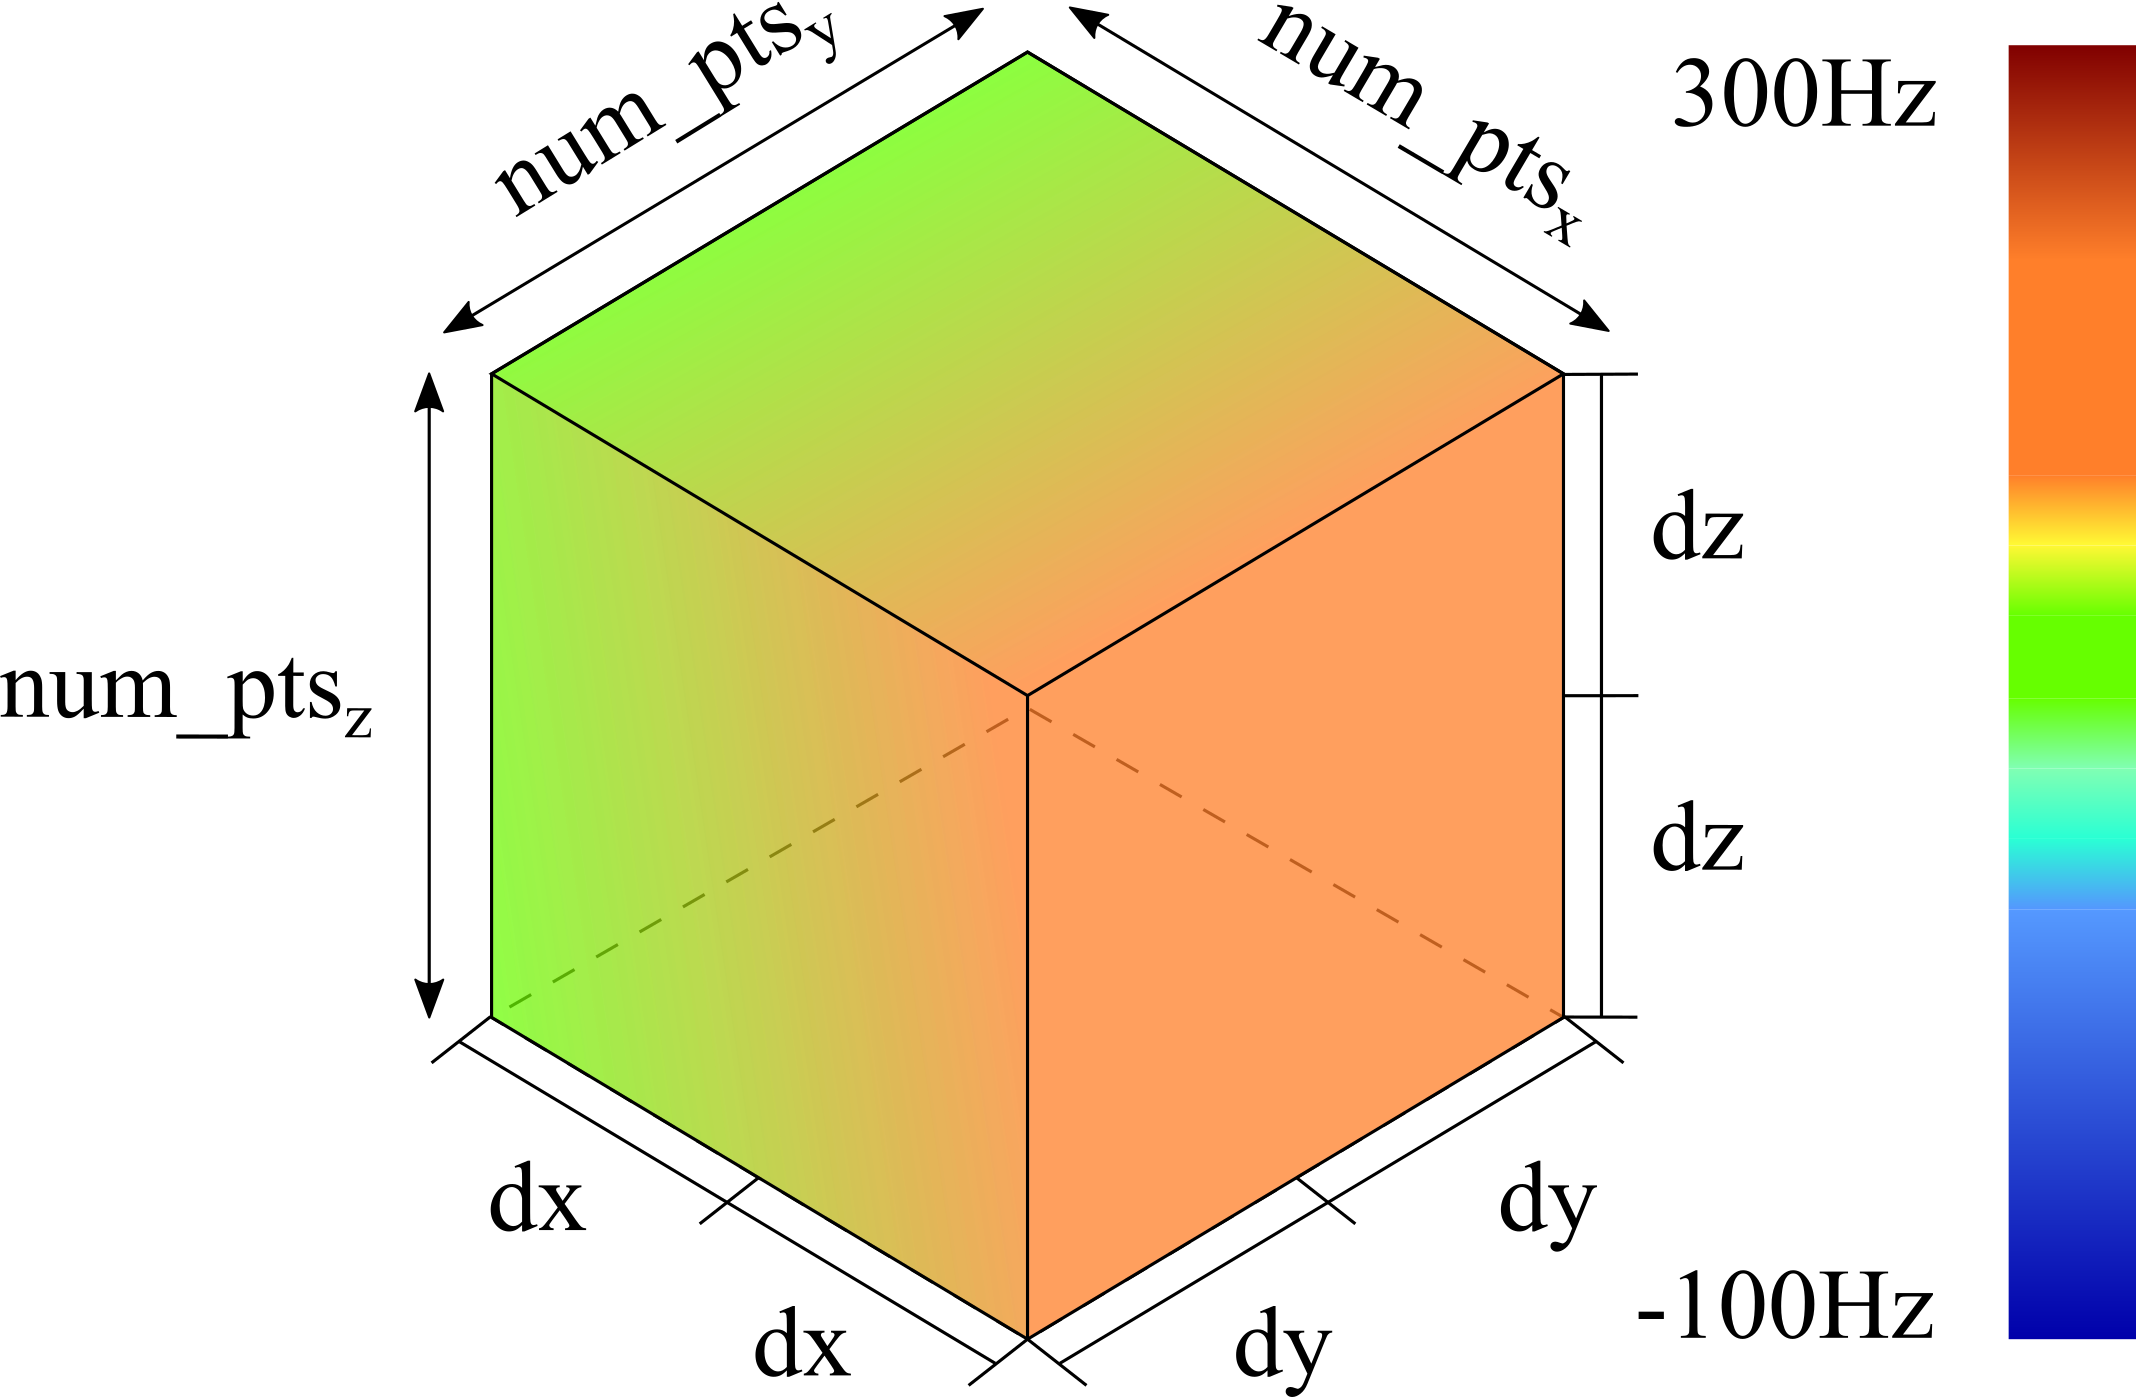
\includegraphics[width=0.5\textwidth]{images/S2:Baseline_exploration/SI_B0_field_model.png}
    \caption{$B_0$ field volume with labels corresponding to the mathematical model for simulating the heterogeneities.}
    \label{fig:SI_B0 model}
\end{figure}

As described in Li et al. \cite{Li2015}, using the $B_0$ field map, measured during the acquisition, to modulate the basis functions prior to fitting showed significant improvement in metabolite quantification and the fit residual surrounding the metabolite peaks. The fact that this technique has a direct impact on metabolite quantification shows the importance of including it when simulating spectra. The first step is to define the spectral and imaging resolutions of the simulated acquisitions. The defaults, shown below, assume a cubic spectroscopy voxel, but any cuboidal shape is acceptable.

\begin{itemize}[labelindent=2cm, widest=spectroscopy voxel, leftmargin=*, align=left] 
    \item[\textbf{spectroscopy voxel}] \textnormal{[10 mm x  10 mm x 10 mm]}
    \item[\textbf{imaging voxel}] \textnormal{[0.5mm x 0.5mm x 0.5mm]}
\end{itemize}

The dimensions of the volume being modeled are the same as the spectroscopy voxel. The number of points included in the simulation is the quotient of spectroscopy resolution and the anatomical imaging resolution.
\begin{equation}
    \mathbf{num\_pts} = \frac{\textnormal{spectroscopy resolution}}{\textnormal{imaging resolution}}
    = \left[{\frac{\textnormal{10mm}}{\textnormal{0.5mm}}}_X, {\frac{\textnormal{10mm}}{\textnormal{0.5mm}}}_Y, {\frac{\textnormal{10mm}}{\textnormal{0.5mm}}}_Z\right]
\end{equation}

Now that the model volume has been defined, it is time to model that actual $B_0$ field, $dB0$. Magnetic fields do not have hard, disjointed heterogeneities, but smooth variations. This is true even in the presence of high susceptibility effects causing strong distortions as long as the voxels are reasonable small. This model therefore assumes linearly varying gradients across the volume of the voxel. This assumption allowed the problem to be reduced to four variables:
\begin{description}[labelindent=2cm]
    \item[$\mathbf{dx}$] half of the mean change in the x-direction
    \item[$\mathbf{dy}$] half of the mean change in the y-direction
    \item[$\mathbf{dz}$] half of the mean change in the z-direction
    \item[$\boldsymbol{\mu\ \ }$] the mean offset of the entire voxel
\end{description}

The next step is to define the gradients in each direction as shown in Eqns. \ref{eqn:dB0_x}, \ref{eqn:dB0_y}, and \ref{eqn:dB0_z}. As mentioned above, this model assumes linearly varying gradients, but more complex gradients can be implemented manually.
\begin{align} 
    &\mathbf{x} = \textnormal{linspace}(\textbf{-dx}, \textbf{dx}, \textbf{num\_pts}_\textnormal{X}) \label{eqn:dB0_x}\\
    &\mathbf{y} = \textnormal{linspace}(\textbf{-dy}, \textbf{dy}, \textbf{num\_pts}_\textnormal{Y}) \label{eqn:dB0_y}\\
    &\mathbf{z} = \textnormal{linspace}(\textbf{-dz}, \textbf{dz}, \textbf{num\_pts}_\textnormal{Z}) \label{eqn:dB0_z}
\end{align}

Once the gradients have been defined, the field map can be modeled very easily, as shown in Eqn. \ref{eqn:calculate dB0}. The primary challenge in this step is reshaping the tensors to get the correct n+3D output.
\begin{align}\label{eqn:calculate dB0}
    &\mathbf{dB0} = \textbf{x}*\textbf{y}*\textbf{z} + \boldsymbol{\mu}\textnormal{, such that}\\ &\mathbf{dB0}.size() = torch.Size([batchSize, …, \textbf{num\_pts}_\textnormal{X}, \textbf{num\_pts}_\textnormal{Y}, \textbf{num\_pts}_\textnormal{Z}])
\end{align}

Modulation due to the heterogeneous magnetic field can be applied in both the time-domain and the frequency-domain. In the time-domain, the complex exponential is applied via multiplication with the basis function, as is shown below in Eqn. \ref{eqn:SI_B0_modulation}. In the frequency-domain, the complex exponential needs to be convolved with the spectrum. In both mathematical and practical terms, it is simpler to apply the modulation in the time-domain.
\begin{equation}\label{eqn:SI_B0_modulation}
    F(t) = \sum_n^N M_n * basisfcn_n * \underbrace{ \sum_{r=1}^R e^{-i\Delta\omega_r t} }_{B_0\ inhomog.} \textnormal{, where }
    \Delta\omega = \mathbf{dB0}.flatten(dims=[-3:-1]) \textnormal{ and } R=cumprod(\textbf{num\_pts})
\end{equation}
In this equation, the model \textbf{dB0} is flattened along the last three dimensions representing the \textbf{x}-, \textbf{y}-, and \textbf{z}-dimensions respectively. Therefore, \textbf{r} represents the linear indices from [1,R] corresponding the subscripts of the points within the 3D volume. The effective magnetic field at each of those points within the voxel has a direct effect on each moeity that resonates and contributes to the overall signal. Because of this, each basis function is modulated independently before summation. 


\newpage
\section{Baseline and Residual Water Simulations}\label{baseline-simulations}
A single simulation protocol is used to generate the contributions for both baseline offsets and residual water contributions. This work uses a smoothed, pseudo-random bounded walk algorithm for the simulations. For simplicity, this will henceforth be referred to as a \emph{(random) bounded walk}, or simply a \emph{walk}. By using different configuration dictionaries, it is possible to switch from very smooth, undulating baselines to rather erratic and rough residual water regions. The following sections highlight the effects different parameters have on the simulations. 

\subsection{Variables}\label{variables}

These simulations use at least 9 degrees of freedom with two additional, but optional, inputs: 
\begin{enumerate}
    \item Starting height (start)
    \item Ending height (end)
    \item Standard deviation of walk (std)
    \item Lower bound (lower)
    \item Upper bound (upper)
    \item Point density (pt\_density)
    \item PPM range (ppm\_range)
    \item Length of smoothing window (window)
    \item Scale (scale)
    \item Dropout probability (drop\_prob)
    \item *Prime (prime)
\end{enumerate}
Floats or integers can be provided for the point density, prime, and drop\_prob. Everything else should be provided as a list with either a single value or a range in the form of [min\_range, max\_range]. When a single value is provided, that variable will be fixed. If a range is specified, then values will be sampled from that range uniformly. The point density and the PPM range are used to calculate the length of the walks. This length coupled with \(std\) control the flexibility of raw simulation. The length of the smoothing window, \(window\), will affect the smoothness of the resulting walk. It is specified as a fraction of the length of the walk, so that it is independent of walk length, and can also be either fixed or sampled. \(scale\) determines how prominent each offset will be when added to the simulated data. \(drop\_prob\) is used to randomly omit the offset from that percentage of the simulations. \(prime\) [units: ppm] is used for generating the residual water regions. This allows the region to vary in length by sampling two values in the range of [\(-prime\),\(prime\)) that can expand, contract, or slightly offset the residual water region.

\subsection{Post-processing}\label{post-processing}
Once the random walks have been generated, they are then smoothed with kernels of either fixed or varying width. At this point, the walks are normalized to [0,1] and then scaled down according to \(scale\). Afterwards, trend lines are calculated between the starting and ending points which are then removed so that they start and end on the x-axis. A function called \emph{sim2acquired} then uses zero padding and a nonuniform interpolater to add tails to both sides of the walks so that they match the PPM range of the basis set regarding the spectral width and carrier frequency. Before being added to the FIDs, they are multiplied by the maximum value of the FID in the frequency domain to scale them up to the correct order of magnitude. This makes \(scale\) relative to the maximum height in the spectra. The offsets are added to the FIDs in the frequency domain before an inverse FFT returns the data to the time domain.

The parameters presented below control the length of the walks, their trend lines, flexibility, and smoothness. The default values presented in the config dictionaries were determined through preliminary experiments to closely approximate what was observed in a clinical dataset.

\subsection{Preparing for the simulations}\label{preparing-for-the-simulations}
The following section defines parameters for the spectroscopy scenario and the config dictionary for the simulations. \\

    \begin{tcolorbox}[breakable, size=fbox, boxrule=1pt, pad at break*=1mm,colback=cellbackground, colframe=cellborder]
\begin{Verbatim}[commandchars=\\\{\}]
\PY{c+c1}{\PYZsh{} Spectroscopy scenario}
\PY{n}{spectralwidth} \PY{o}{=} \PY{l+m+mi}{2000}                       \PY{c+c1}{\PYZsh{} Hz}
\PY{n}{Ns}            \PY{o}{=} \PY{l+m+mi}{2048}                       \PY{c+c1}{\PYZsh{} number of spectral points}
\PY{n}{B0}            \PY{o}{=} \PY{l+m+mf}{3.0}                        \PY{c+c1}{\PYZsh{} T}
\PY{n}{gamma\PYZus{}H}       \PY{o}{=} \PY{l+m+mf}{42.577478518}               \PY{c+c1}{\PYZsh{} MHz/T}
\PY{n}{ppm\PYZus{}ref}       \PY{o}{=} \PY{l+m+mf}{4.65}                       \PY{c+c1}{\PYZsh{} ppm}

\PY{n}{carrier\PYZus{}frequency} \PY{o}{=} \PY{n}{B0} \PY{o}{*} \PY{n}{gamma\PYZus{}H}           \PY{c+c1}{\PYZsh{} MHz}
\PY{n}{ppm} \PY{o}{=} \PY{n}{torch}\PY{o}{.}\PY{n}{linspace}\PY{p}{(}\PY{o}{\PYZhy{}}\PY{l+m+mf}{0.5}\PY{o}{*}\PY{n}{spectralwidth}\PY{p}{,}   
                     \PY{l+m+mf}{0.5}\PY{o}{*}\PY{n}{spectralwidth}\PY{p}{,}\PY{n}{Ns}\PY{p}{)} \PY{c+c1}{\PYZsh{} Hz}
\PY{n}{ppm} \PY{o}{/}\PY{o}{=} \PY{n}{carrier\PYZus{}frequency}                   \PY{c+c1}{\PYZsh{} ppm}
\PY{n}{ppm} \PY{o}{+}\PY{o}{=} \PY{n}{ppm\PYZus{}ref}
\PY{n}{t} \PY{o}{=} \PY{n}{torch}\PY{o}{.}\PY{n}{linspace}\PY{p}{(}\PY{l+m+mi}{0}\PY{p}{,}\PY{n}{Ns}\PY{o}{/}\PY{n}{spectralwidth}\PY{p}{,}\PY{n}{Ns}\PY{p}{)}

\PY{n}{num\PYZus{}samples} \PY{o}{=} \PY{l+m+mi}{10}
\end{Verbatim}
\end{tcolorbox}


\subsection{Understanding the Simulation Plots}
The plots below follow contain either one or two lines that are blue or red. The default color scheme is as follows:
\begin{itemize}[labelindent=2cm, widest=blue, leftmargin=*, align=left]
    \item[\textbf{\textcolor{pltblue}{blue}}] raw random walk simulation
    \item[\textbf{\textcolor{pltred}{red}}] smoothed walk that is added to the simulated spectra
\end{itemize}
In Sections \ref{baseline:incorporating-the-offsets-into-the-spectra} and \ref{reswater:incorporating-the-offsets-into-the-spectra}, which discuss how to incorporate the walks into the simulated spectra, only a single blue line is plotted. This line is the smoothed, real component of the walk. In Sections \ref{baseline:effect-of-the-hilbert-transform} and \ref{reswater:effect-of-the-hilbert-transform} which show the effect of applying the Hilbert transform, the blue and red lines represent the real and imaginary components, respectively. Similarly, Sections \ref{baseline:compiled-generator} and \ref{reswater:compiled-generator}, which include examples of random simulations for each contribution type, also show the real and imaginary components using the blue and red, respectively.

\newpage
\subsection{Baseline Offsets}\label{baseline-offsets}
The following section will explore this generator using the baseline configuration dictionary defined below. The values selected for the plots in the following sections were tailored specifically to the baseline simulations.\\

    \begin{tcolorbox}[breakable, size=fbox, boxrule=1pt, pad at break*=1mm,colback=cellbackground, colframe=cellborder]

\begin{Verbatim}[commandchars=\\\{\}]
\PY{n}{baseline\PYZus{}cfg} \PY{o}{=} \PY{p}{\PYZob{}}
        \PY{l+s+s2}{\PYZdq{}}\PY{l+s+s2}{start}\PY{l+s+s2}{\PYZdq{}}\PY{p}{:}           \PY{p}{[}    \PY{o}{\PYZhy{}}\PY{l+m+mi}{1}\PY{p}{,}     \PY{l+m+mi}{1}\PY{p}{]}\PY{p}{,}
        \PY{l+s+s2}{\PYZdq{}}\PY{l+s+s2}{end}\PY{l+s+s2}{\PYZdq{}}\PY{p}{:}             \PY{p}{[}    \PY{o}{\PYZhy{}}\PY{l+m+mi}{1}\PY{p}{,}     \PY{l+m+mi}{1}\PY{p}{]}\PY{p}{,}
        \PY{l+s+s2}{\PYZdq{}}\PY{l+s+s2}{upper}\PY{l+s+s2}{\PYZdq{}}\PY{p}{:}           \PY{p}{[}            \PY{l+m+mi}{1}\PY{p}{]}\PY{p}{,}
        \PY{l+s+s2}{\PYZdq{}}\PY{l+s+s2}{lower}\PY{l+s+s2}{\PYZdq{}}\PY{p}{:}           \PY{p}{[}           \PY{o}{\PYZhy{}}\PY{l+m+mi}{1}\PY{p}{]}\PY{p}{,}
        \PY{l+s+s2}{\PYZdq{}}\PY{l+s+s2}{std}\PY{l+s+s2}{\PYZdq{}}\PY{p}{:}             \PY{p}{[}  \PY{l+m+mf}{0.05}\PY{p}{,}  \PY{l+m+mf}{0.20}\PY{p}{]}\PY{p}{,}
        \PY{l+s+s2}{\PYZdq{}}\PY{l+s+s2}{window}\PY{l+s+s2}{\PYZdq{}}\PY{p}{:}          \PY{p}{[}  \PY{l+m+mf}{0.15}\PY{p}{,}   \PY{l+m+mf}{0.3}\PY{p}{]}\PY{p}{,}
        \PY{l+s+s2}{\PYZdq{}}\PY{l+s+s2}{pt\PYZus{}density}\PY{l+s+s2}{\PYZdq{}}\PY{p}{:}          \PY{l+m+mi}{128}\PY{p}{,}
        \PY{l+s+s2}{\PYZdq{}}\PY{l+s+s2}{ppm\PYZus{}range}\PY{l+s+s2}{\PYZdq{}}\PY{p}{:}       \PY{p}{[}  \PY{o}{\PYZhy{}}\PY{l+m+mf}{1.6}\PY{p}{,}   \PY{l+m+mf}{8.5}\PY{p}{]}\PY{p}{,}
        \PY{l+s+s2}{\PYZdq{}}\PY{l+s+s2}{scale}\PY{l+s+s2}{\PYZdq{}}\PY{p}{:}           \PY{p}{[}     \PY{l+m+mi}{0}\PY{p}{,}   \PY{l+m+mf}{1}\PY{p}{]}\PY{p}{,}
        \PY{l+s+s2}{\PYZdq{}}\PY{l+s+s2}{drop\PYZus{}prob}\PY{l+s+s2}{\PYZdq{}}\PY{p}{:}           \PY{l+m+mf}{0.0}
\PY{p}{\PYZcb{}}
\end{Verbatim}
\end{tcolorbox}

\subsubsection{Standard Deviation}\label{baseline:standard-deviation}
This section shows the effect of different std values on the random walk. The \(std\) variable is used when sampling the noise for the walk. It directly controls the amount of variation between two consecutive points prior to the cumulative summation.

\begin{center}
    \newpage 
Standard Deviation :: STD = 0.05; Window length = random; Kernel\_size = random; Point density = 128


    \begin{center}
    \adjustimage{max size={0.85\linewidth}{0.85\paperheight}}{images/S2:Baseline_exploration/output_14_1.png}
    \end{center}

    
    \newpage

Standard Deviation :: STD = 0.10; Window length = random; Kernel\_size = random; Point density = 128


    \begin{center}
    \adjustimage{max size={0.85\linewidth}{0.85\paperheight}}{images/S2:Baseline_exploration/output_14_3.png}
    \end{center}

    
    \newpage 
Standard Deviation :: STD = 0.15; Window length = random; Kernel\_size = random; Point density = 128


    \begin{center}
    \adjustimage{max size={0.85\linewidth}{0.85\paperheight}}{images/S2:Baseline_exploration/output_14_5.png}
    \end{center}

    
    \newpage 
Standard Deviation :: STD = 0.20; Window length = random; Kernel\_size = random; Point density = 128


    \begin{center}
    \adjustimage{max size={0.85\linewidth}{0.85\paperheight}}{images/S2:Baseline_exploration/output_14_7.png}
    \end{center}

\end{center}
    
\newpage
\subsubsection{Smoothing Kernel}\label{baseline:smoothing-kernel}
In this section, the effects of different smoothing kernel lengths are explored given a fixed $std$ value.

\begin{center}
Smoothing Kernel :: STD = 0.10; Window Length = 0.10, Kernel\_size = 60; Point density = 128


    \begin{center}
    \adjustimage{max size={0.85\linewidth}{0.85\paperheight}}{images/S2:Baseline_exploration/output_16_1.png}
    \end{center}

    
    \newpage 
Smoothing Kernel :: STD = 0.10; Window Length = 0.20, Kernel\_size = 120; Point density = 128


    \begin{center}
    \adjustimage{max size={0.85\linewidth}{0.85\paperheight}}{images/S2:Baseline_exploration/output_16_3.png}
    \end{center}

    
    \newpage 
Smoothing Kernel :: STD = 0.10; Window Length = 0.30, Kernel\_size = 180; Point density = 128


    \begin{center}
    \adjustimage{max size={0.85\linewidth}{0.85\paperheight}}{images/S2:Baseline_exploration/output_16_5.png}
    \end{center}

\end{center}
    
\newpage
\subsubsection{Point Density}\label{baseline:point-density}
This section explores the effect of varying the point density of the random walk while keeping the \(std\) fixed. Results are presented using two different kernel sizes for the smoothing.

\begin{center}
Point Density :: STD = 0.10, Window Length = [0.10, 0.30], Kernel\_size = [3,9]; Point density = 64


    \begin{center}
    \adjustimage{max size={0.84\linewidth}{0.84\paperheight}}{images/S2:Baseline_exploration/output_18_1.png}
    \end{center}

    
    \newpage 
Point Density :: STD = 0.10, Window Length = [0.10, 0.30], Kernel\_size = [3,9]; Point density = 128


    \begin{center}
    \adjustimage{max size={0.85\linewidth}{0.85\paperheight}}{images/S2:Baseline_exploration/output_18_3.png}
    \end{center}

    
    \newpage 
Point Density :: STD = 0.10, Window Length = [0.10, 0.30], Kernel\_size = [3,9]; Point density = 256


    \begin{center}
    \adjustimage{max size={0.85\linewidth}{0.85\paperheight}}{images/S2:Baseline_exploration/output_18_5.png}
    \end{center}

\end{center}
    
\newpage
\subsubsection{Incorporating the offsets into the spectra}\label{baseline:incorporating-the-offsets-into-the-spectra}
To increase variability, the starting and ending heights are randomly selected. When considering the entire spectrum, however, these must be adjusted to avoid unrealistic, hard transition points.

\begin{center}
With the original trend lines still included


    \begin{center}
    \adjustimage{max size={0.84\linewidth}{0.84\paperheight}}{images/S2:Baseline_exploration/output_20_1.png}
    \end{center}

    
    \newpage 
With the original trend lines removed


    \begin{center}
    \adjustimage{max size={0.85\linewidth}{0.85\paperheight}}{images/S2:Baseline_exploration/output_20_3.png}
    \end{center}
    { \hspace*{\fill} \\}
\end{center}

\newpage
\subsubsection{Effect of the Hilbert Transform}\label{baseline:effect-of-the-hilbert-transform}
Simulating spectra requires complex spectral components, including the baseline and residual water. The Hilbert transform is used to generate those corresponding imaginary components. 

    \begin{center}
    \adjustimage{max size={0.85\linewidth}{0.85\paperheight}}{images/S2:Baseline_exploration/output_22_0.png}
    \end{center}


\newpage
\subsubsection{Compiled Generator}\label{baseline:compiled-generator}
This shows the variety of baselines that can be generated when randomly sampling all variables.
    \begin{center}
    \adjustimage{max size={0.85\linewidth}{0.85\paperheight}}{images/S2:Baseline_exploration/output_26_0.png}
    \end{center}

\newpage
\subsection{Residual Water}\label{residual-water}

The following section will explore this generator using the residual water dictionary defined below. While the sections are the same as in Sec. \ref{baseline-offsets}, the values displayed are tailored to the ranges for the residual water simulations.

\subsubsection{Configuration dictionaries}\label{configuration-dictionaries}
The following dictionaries are the standard defaults in MRS-Sim for generating baseline offsets and residual water contributions. To explore how the models output change with the different dictionaries, toggle between the two cfg options in the Section \ref{preparing-for-the-simulations} below.\\

    \begin{tcolorbox}[breakable, size=fbox, boxrule=1pt, pad at break*=1mm,colback=cellbackground, colframe=cellborder]
\begin{Verbatim}[commandchars=\\\{\}]
\PY{n}{resWater\PYZus{}cfg} \PY{o}{=} \PY{p}{\PYZob{}}
        \PY{l+s+s2}{\PYZdq{}}\PY{l+s+s2}{start}\PY{l+s+s2}{\PYZdq{}}\PY{p}{:}           \PY{p}{[}            \PY{l+m+mi}{0}\PY{p}{]}\PY{p}{,}
        \PY{l+s+s2}{\PYZdq{}}\PY{l+s+s2}{end}\PY{l+s+s2}{\PYZdq{}}\PY{p}{:}             \PY{p}{[}            \PY{l+m+mi}{0}\PY{p}{]}\PY{p}{,}
        \PY{l+s+s2}{\PYZdq{}}\PY{l+s+s2}{upper}\PY{l+s+s2}{\PYZdq{}}\PY{p}{:}           \PY{p}{[}     \PY{l+m+mi}{0}\PY{p}{,}     \PY{l+m+mi}{1}\PY{p}{]}\PY{p}{,}
        \PY{l+s+s2}{\PYZdq{}}\PY{l+s+s2}{lower}\PY{l+s+s2}{\PYZdq{}}\PY{p}{:}           \PY{p}{[}     \PY{l+m+mi}{0}\PY{p}{,}     \PY{l+m+mi}{1}\PY{p}{]}\PY{p}{,}
        \PY{l+s+s2}{\PYZdq{}}\PY{l+s+s2}{std}\PY{l+s+s2}{\PYZdq{}}\PY{p}{:}             \PY{p}{[}   \PY{l+m+mf}{0.2}\PY{p}{,}  \PY{l+m+mf}{0.40}\PY{p}{]}\PY{p}{,}
        \PY{l+s+s2}{\PYZdq{}}\PY{l+s+s2}{window}\PY{l+s+s2}{\PYZdq{}}\PY{p}{:}          \PY{p}{[}  \PY{l+m+mf}{0.05}\PY{p}{,}  \PY{l+m+mf}{0.15}\PY{p}{]}\PY{p}{,}
        \PY{l+s+s2}{\PYZdq{}}\PY{l+s+s2}{pt\PYZus{}density}\PY{l+s+s2}{\PYZdq{}}\PY{p}{:}         \PY{l+m+mi}{1204}\PY{p}{,}
        \PY{l+s+s2}{\PYZdq{}}\PY{l+s+s2}{ppm\PYZus{}range}\PY{l+s+s2}{\PYZdq{}}\PY{p}{:}       \PY{p}{[}   \PY{l+m+mf}{4.4}\PY{p}{,}   \PY{l+m+mf}{4.9}\PY{p}{]}\PY{p}{,}
        \PY{l+s+s2}{\PYZdq{}}\PY{l+s+s2}{prime}\PY{l+s+s2}{\PYZdq{}}\PY{p}{:}              \PY{l+m+mf}{0.15}\PY{p}{,}
        \PY{l+s+s2}{\PYZdq{}}\PY{l+s+s2}{scale}\PY{l+s+s2}{\PYZdq{}}\PY{p}{:}           \PY{p}{[}   \PY{l+m+mf}{1.0}\PY{p}{,}   \PY{l+m+mf}{1.0}\PY{p}{]}\PY{p}{,} \PY{c+c1}{\PYZsh{} typically: [0.05, 0.20] - better visualization.}
        \PY{l+s+s2}{\PYZdq{}}\PY{l+s+s2}{drop\PYZus{}prob}\PY{l+s+s2}{\PYZdq{}}\PY{p}{:}           \PY{l+m+mf}{0.0}
\PY{p}{\PYZcb{}}
\end{Verbatim}
\end{tcolorbox}

\subsubsection{Standard Deviation}\label{standard-deviation}\raggedright
This section shows the effect of different std values on the random walk. The \(std\) variable is used when sampling the noise for the walk. It directly controls the amount of variation between two consecutive points prior to the cumulative summation.

    \newpage 
    \begin{center} 
Standard Deviation :: STD = 0.20; Window length = random; Kernel\_size = random; Point density = 1204


    \begin{center}
    \adjustimage{max size={0.85\linewidth}{0.85\paperheight}}{images/S2:Baseline_exploration/output_30_1.png}
    \end{center}
    { \hspace*{\fill} \\}
    
    \newpage 
Standard Deviation :: STD = 0.30; Window length = random; Kernel\_size = random; Point density = 1204

    \begin{center}
    \adjustimage{max size={0.85\linewidth}{0.85\paperheight}}{images/S2:Baseline_exploration/output_30_3.png}
    \end{center}
    { \hspace*{\fill} \\}
    
    \newpage 
Standard Deviation :: STD = 0.40; Window length = random; Kernel\_size = random; Point density = 1204


    \begin{center}
    \adjustimage{max size={0.85\linewidth}{0.85\paperheight}}{images/S2:Baseline_exploration/output_30_5.png}
    \end{center}
    { \hspace*{\fill} \\}
    
    \newpage 
Standard Deviation :: STD = 0.50; Window length = random; Kernel\_size = random; Point density = 1204


    \begin{center}
    \adjustimage{max size={0.85\linewidth}{0.85\paperheight}}{images/S2:Baseline_exploration/output_30_7.png}
    \end{center}
    { \hspace*{\fill} \\}
\end{center}
    
\subsubsection{Smoothing Kernel}\label{reswater:smoothing-kernel}\raggedright
In this section, the effects of different smoothing kernel lengths are explored given a fixed $std$ value.

\begin{center}
Smoothing Kernel :: STD = 0.10, Window Length = 0.05, Kernel\_size = 30; Point density = 1204


    \begin{center}
    \adjustimage{max size={0.85\linewidth}{0.85\paperheight}}{images/S2:Baseline_exploration/output_32_1.png}
    \end{center}

    
    \newpage 
Smoothing Kernel :: STD = 0.10, Window Length = 0.10, Kernel\_size = 60; Point density = 1204


    \begin{center}
    \adjustimage{max size={0.85\linewidth}{0.85\paperheight}}{images/S2:Baseline_exploration/output_32_3.png}
    \end{center}
    { \hspace*{\fill} \\}
    
    \newpage 
Smoothing Kernel :: STD = 0.10, Window Length = 0.15, Kernel\_size = 90; Point density = 1204



    \begin{center}
    \adjustimage{max size={0.85\linewidth}{0.85\paperheight}}{images/S2:Baseline_exploration/output_32_5.png}
    \end{center}
    { \hspace*{\fill} \\}
\end{center}

\subsubsection{Point Density}\label{reswater:point-density}\raggedright
This section explores the effect of varying the point density of the random walk while keeping the \(std\) fixed. Results are presented using two different kernel sizes for the smoothing.

    
\begin{center}
Point Density :: STD = 0.10, Window Length = [0.05, 0.15], Kernel\_size = [12,38]; Point density = 512


    \begin{center}
    \adjustimage{max size={0.84\linewidth}{0.84\paperheight}}{images/S2:Baseline_exploration/output_34_1.png}
    \end{center}
    
    \newpage 
Point Density :: STD = 0.10, Window Length = [0.05, 0.15], Kernel\_size = [12,38]; Point density = 1024


    \begin{center}
    \adjustimage{max size={0.85\linewidth}{0.85\paperheight}}{images/S2:Baseline_exploration/output_34_3.png}
    \end{center}
    { \hspace*{\fill} \\}
    
    \newpage 
Point Density :: STD = 0.10, Window Length = [0.05, 0.15], Kernel\_size = [12,38]; Point density = 2048


    \begin{center}
    \adjustimage{max size={0.85\linewidth}{0.85\paperheight}}{images/S2:Baseline_exploration/output_34_5.png}
    \end{center}
    { \hspace*{\fill} \\}
\end{center}
    
\subsubsection{Incorporating the offsets into the spectra}\label{reswater:incorporating-the-offsets-into-the-spectra}\raggedright
To increase variability, the starting and ending heights are randomly selected. When considering the entire spectrum, however, these must be adjusted to avoid unrealistic, hard transition points.

    % \begin{Verbatim}[commandchars=\\\{\}]
\begin{center}
With the original trend lines still included


    \begin{center}
    \adjustimage{max size={0.84\linewidth}{0.84\paperheight}}{images/S2:Baseline_exploration/output_36_1.png}
    \end{center}

    
\newpage
With the original trend lines removed


    \begin{center}
    \adjustimage{max size={0.85\linewidth}{0.85\paperheight}}{images/S2:Baseline_exploration/output_36_3.png}
    \end{center}

\end{center}

\subsubsection{Effect of the Hilbert Transform}\label{reswater:effect-of-the-hilbert-transform}%\raggedright
Simulating spectra requires complex spectral components, including the baseline and residual water. The Hilbert transform is used to generate those corresponding imaginary components. 

    \begin{center}
    \adjustimage{max size={0.85\linewidth}{0.85\paperheight}}{images/S2:Baseline_exploration/output_38_0.png}
    \end{center}


    
\subsubsection{Compiled Generator}\label{reswater:compiled-generator}\raggedright
This shows the variety of residual water contributions that can be generated when randomly sampling all variables.

    \begin{center}
    \adjustimage{max size={0.85\linewidth}{0.85\paperheight}}{images/S2:Baseline_exploration/output_42_0.png}
    \end{center}
    { \hspace*{\fill} \\}
    

    
\end{document}
